\section{Introduction}
In this chapter the design method, seen on \cref{scenarioModel} is followed to create the interaction design for the program. The method focuses on the use of scenarios, which are about people performing activities in context by using technology, throughout the design process. In the model there are different design processes shown as clouds and the products of these processes shown as the square boxes. Each of the main processes; Understanding, Envisionment, Evaluation and Design, in designing interactive systems are used in the scenario based method. The figure, \cref{scenarioModel} is rather complex and has therefore, in this report, been split into three sections, \nameref{ModDev} in \ref{ModDev}, \nameref{ProtDev} in \ref{ProtDev} and \nameref{DesDev} in \ref{DesDev}. \nameref{ModDev} uses the product \textit{User stories} and \textit{Conceptual model}, are processed with the \textit{Understanding} Process, to create the products; \textit{Requirements} and \textit{Scenario corpus}, which then are used to create the final product of this section, a \textit{Conceptual model}. The second section, \nameref{ProtDev}, a new product, \textit{Concrete scenarios} is created from \textit{Conceptual scenarios}, \textit{Concrete scenarios} are then processed to create paper prototypes. Lastly the third section, \nameref{DesDev} combines the two previous sections, to define a \textit{Design language}.

\begin{figure}[H]
	\centering
	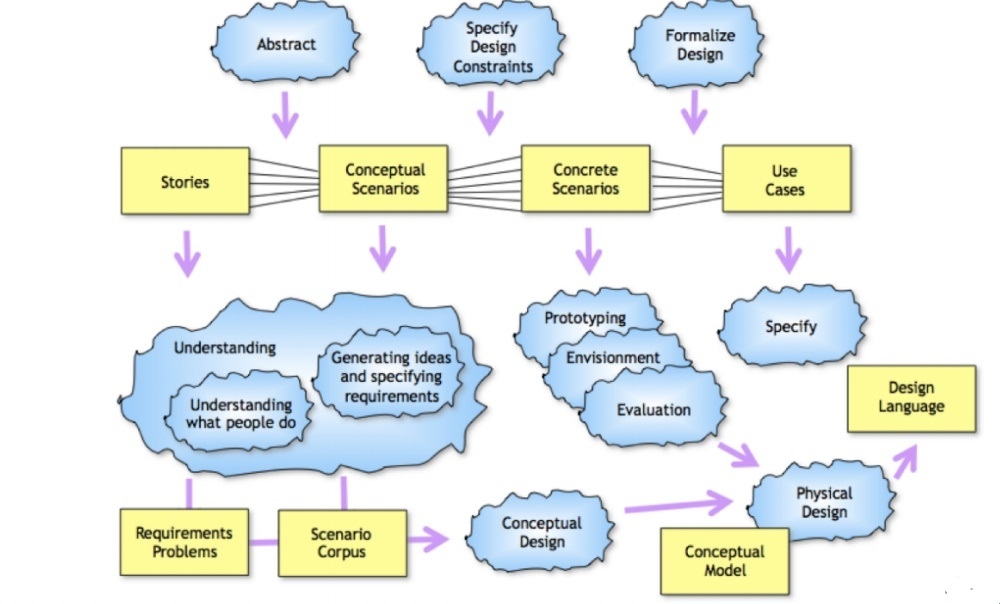
\includegraphics[width=1\textwidth]{Grafik/scenarioModel}
	\caption{Scenario-based design method}
	\label{scenarioModel}
\end{figure}